\begin{figure}[tb]
  \centering
\begin{tikzpicture}

  % définition des styles
  \tikzstyle{gw}=[draw]
  \tikzstyle{visible}=[draw]
  \tikzstyle{router}=[circle, draw, fill=orange!50,text=black]
  \tikzstyle{child}=[circle, draw, fill=yellow!50,text=black]
  \tikzstyle{root}=[circle, draw, fill=red!50,text=black]
  %\tikzstyle{node}=[circle, draw, fill=yellow!50,text=black]

  % les nœuds
  \node[gw, ] (gw) at (0, 0) {Passerelle};

  \node[visible, above=1.5cm of gw] (supervision) {Supervision};
  \node[visible, right=1cm of supervision] (selection) {Selection};
  \node[visible, left=1cm of supervision] (estimation) {Estimation};

  % Réseau contraint
  %\node[root] (1) at (-2, 0) {};
  %\node[router] (2) at (-4, 1) {};
  %\node[child] (3) at (-4, -1) {};
  %\node[child] (4) at (-5, 2) {};
  %\node[child] (5) at (-5, 0) {};

  \node[cloud, cloud puffs = 10, cloud ignores aspect, minimum height=2cm,
  minimum width = 4cm, draw, right=1cm of gw, fill = gray!10] (cloud)
  {Internet};

  \node[cloud, cloud puffs = 10, cloud ignores aspect, minimum height=2cm,
  minimum width = 4cm, draw, left=1cm of gw, fill = gray!10] (lln) {LoWPAN};

\path
  % Réseau conventionnel
  (gw.east) edge[<->, very thick, green] (cloud)
  (lln) edge[<->, very thick, green] (gw.west)
  (supervision) edge[<->, red, thick, dashed, bend left] (lln.east)

  % Supervision
  (selection) edge[->, ] (supervision)
  (supervision) edge[<-, thick, green, ] (gw)
  (estimation) edge[<->, thick, red] (supervision)
  (supervision) edge[<->, thick, red] (selection)

  ;

  \node[above=0.1cm of estimation](estimationanchor){};
  \node[above=0.1cm of supervision](supervisionanchor){};
  \node[above=0.1cm of selection](selectionanchor){};

  \draw [decorate,decoration={brace,amplitude=10pt,raise=4pt},yshift=0pt]
  (estimationanchor) -- (selectionanchor) node [black,midway,yshift=1cm] {\footnotesize Cycle d'apprentissage};

  \end{tikzpicture}

  \caption{Supervision et sélection de nœuds}

  \label{supervision:fig:schema}
\end{figure}

% Nous utiliserons les données présentées dans la Table~\ref{supervision:table:datasheet} pour calculer l'énergie consommée.

% \begin{table}
%   \centering
%   \begin{tabular}[ht]{|c|c|}
%     \hline
%     \textbf{Tension d'alimentation} & 3.6 V \\ \hline
%     \textbf{MCU on, Radio RX} & 21.8 mA \\ \hline
%     \textbf{MCU on, Radio TX} & 19.5 mA \\ \hline
%     \textbf{MCU on, Radio off} & 1800 $\mu$A \\ \hline
%     \textbf{MCU standby} & 5.1 $\mu$A \\ \hline
%     \textbf{MCU idle, Radio off} & 54.5 $\mu$A \\ \hline
%   \end{tabular}
%   \caption{Consommation énergétique du Tmote sky}
%   \label{supervision:table:datasheet}
% \end{table}

\begin{figure}[tb]
  \centering
  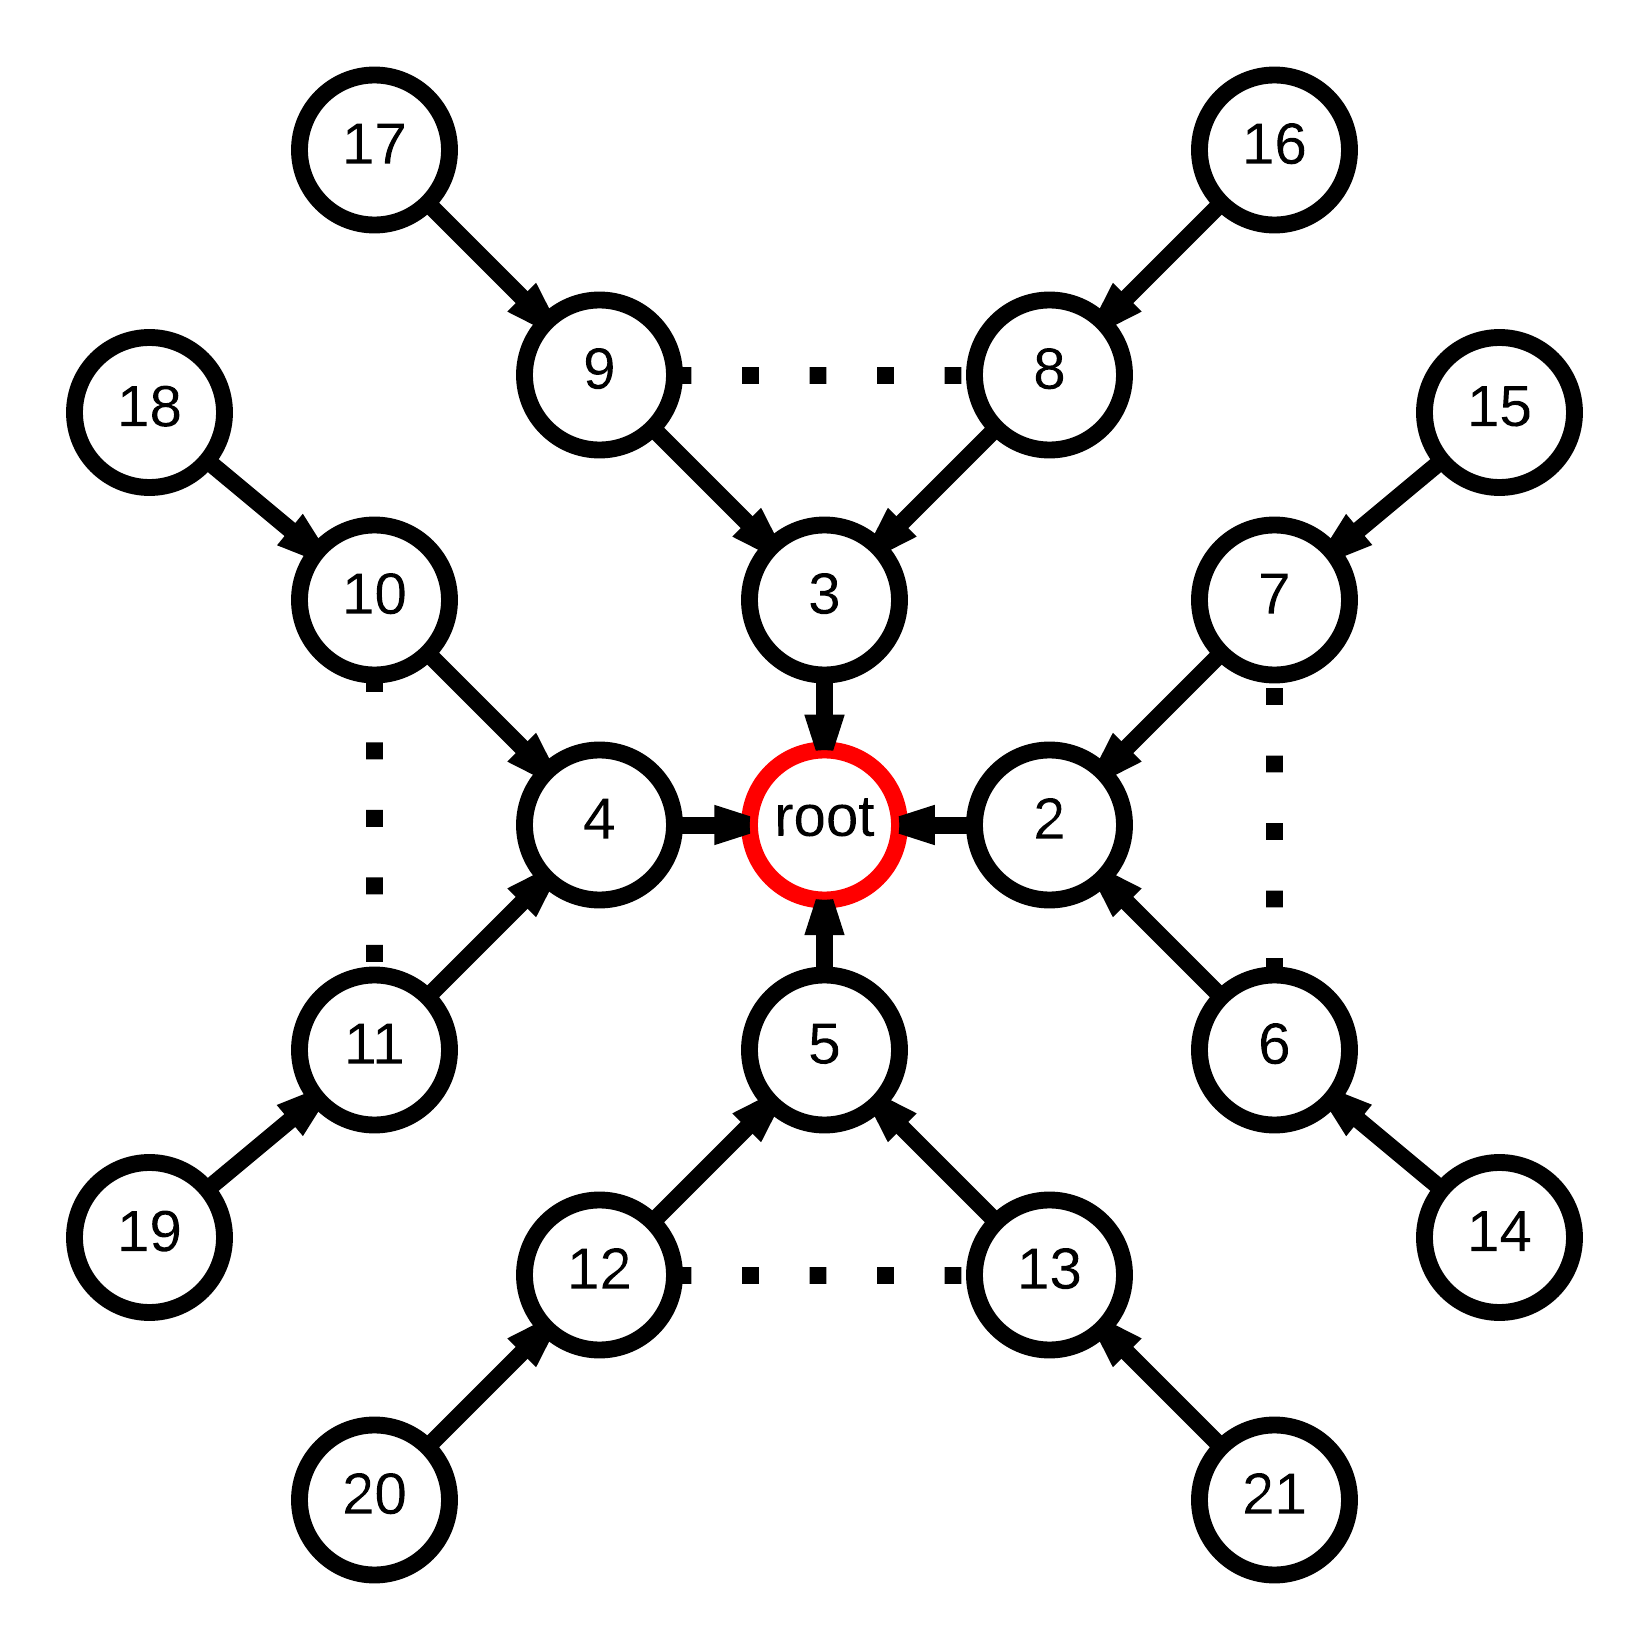
\includegraphics[width=0.5\textwidth]{img/topology_tree.png}
  \caption{Topologie réseau et radio.}
  \label{supervision:fig:topology_tree}
\end{figure}

% Nous avons pris la valeur de $\alpha = 0.25$ afin de ne pas réagir trop brusquement aux pics de trafic brusques causés par une reconstruction du \ac{DODAG} \ac{RPL} qui sont courants lorsque ContikiMAC est utilisé.

% Il peut être calculé en utilisant une \ac{EWMA}, comme montré dans l'équation~\ref{supervision:eqn:bias}.
% Au temps t $t$, cette erreur est prise proportionnellement au temps depuis la dernière supervision active qui se produit tous les $T$.

% TODO: Ajouter une mention à l'équation explicitement.

% \begin{figure}[ht]
%   \begin{subfigure}{0.5\textwidth}
%     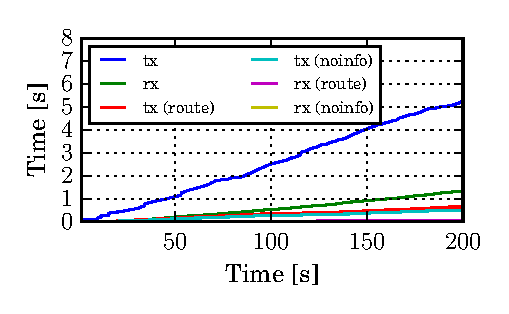
\includegraphics[width=\textwidth]{img/series_cost_3.pdf}
%     \caption{Supervision passive pour le noeud 3}
%     \label{supervision:fig:node3}
%   \end{subfigure}
%   \begin{subfigure}{0.5\textwidth}
%     \centering
%     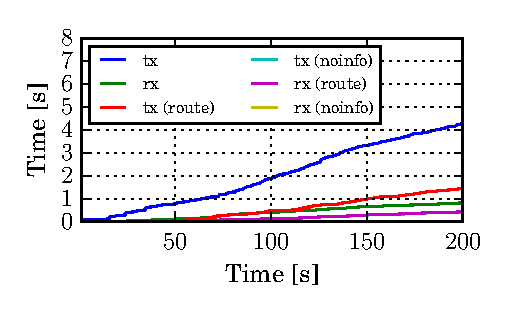
\includegraphics[width=\textwidth]{img/series_cost_5.pdf}
%     \caption{Supervision passive pour le noeud 5}
%     \label{supervision:fig:node5}
%   \end{subfigure}%
% \end{figure}

% \begin{figure*}
%   \centering
%   \begin{subfigure}{0.7\textwidth}
%     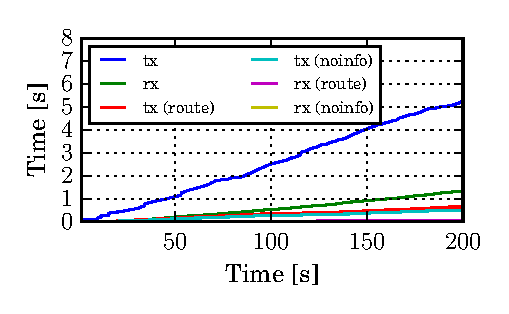
\includegraphics[width=\textwidth]{img/series_cost_3.pdf}
%     \caption{Nœud 3}
%   \end{subfigure}%
%   \begin{subfigure}{0.7\textwidth}
%     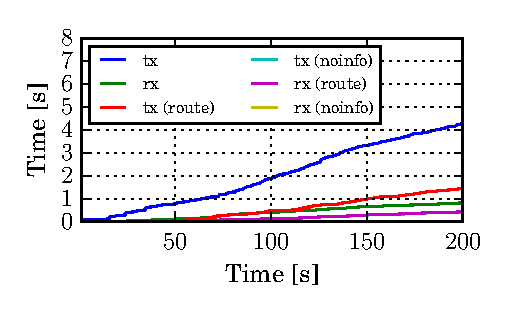
\includegraphics[width=\textwidth]{img/series_cost_5.pdf}
%     \caption{Nœud 5}
%   \end{subfigure}%
%   \begin{subfigure}{0.7\textwidth}
%     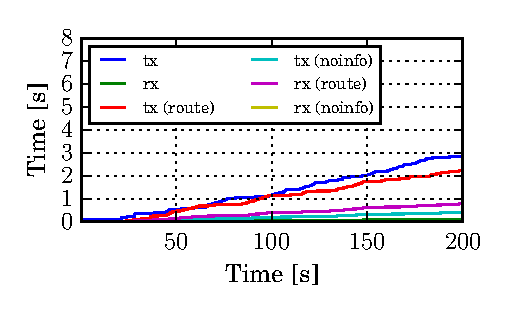
\includegraphics[width=\textwidth]{img/series_cost_7.pdf}
%     \caption{Nœud 7}
%   \end{subfigure}
%   \caption{Cout estimé dans les scénarios de chaines}
%   \label{supervision:fig:chain_experiment}
% \end{figure*}

% \begin{figure}[!ht]
%   \centering
%   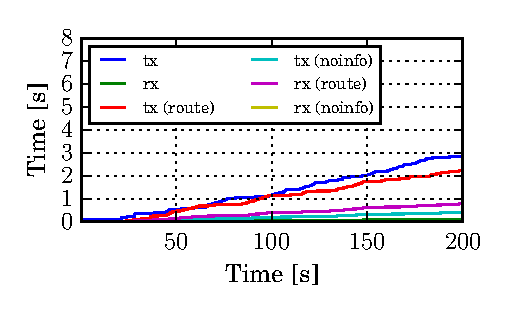
\includegraphics[width=.7\textwidth]{img/series_cost_7.pdf}
%   \caption{Estimation pour un noeud ``feuille''}
%   \label{supervision:fig:node7}
% \end{figure}

% \subsection{Mesure active pour la correction des biais}
% \label{supervision:active_estimation}


% Nous observons que les estimations de transmission divergent beaucoup plus que les estimations de réception.
% C'est cohérent avec les résultats montrés dans la figure~\ref{supervision:fig:average_strobing} car dans ContikiMAC, un noeud source envoie plusieurs fois un paquet avant qu'il ne soit reçu.
% Ainsi les nœuds passent plus de temps à transmettre qu'à recevoir donc le biais d'estimation est plus fort pour la transmission que pour la réception.

\subsubsection{Déduction de l'énergie consommée}

Soit $P_{\tx{}}$ et $P_{\rx{}}$ les puissances utilisées par la radio d'un nœud pour émettre et recevoir respectivement.
L'énergie dépensée pour transmettre est $P_{\tx{}} * T_p(f)$ et respectivement $P_{\rx{}} * T_p(f)$ pour recevoir.

Ces paramètres peuvent être trouvés dans les notices d'utilisations des composants utilisés. 
Par exemple, la radio Chipcon CC2420~\cite{chipcon} implémentant \ieee{} opère avec une tension de $V_{\textrm{DD}} = 3V$, le courant pendant la réception est de $I_{\rx{}} = 19.7\,mA$ et le courant durant une émission à 0\,dBm est $I_{\tx{}} = 17.4\,mA$~\cite{cc2420datasheet}.

Ainsi il est possible d'estimer $S_{\textrm{cost}}(f)$ et $R_{\textrm{cost}}(f)$, l'énergie nécessaire pour respectivement envoyer et recevoir une trame $f$:

\begin{align}
  S_{\textrm{cost}}(f) &= P_{\tx{}}  N_{\textrm{sender}}(f)  T_p(f) +  P_{\rx{}}  t(ACK)\\
  R_{\textrm{cost}}(f) &= P_{\rx{}}  N_{\textrm{receiver}}(f)  T_p(f) + P_{\tx{}}  t(ACK)
\end{align}

où $N_{\textrm{sender}}(f)$ et $N_{\textrm{receiver}}(f)$ sont le nombre de tentatives entreprises par l'expéditeur et le destinataire respectivement. 

Dans le reste du scénario, le trafic réseau est considéré comme suffisamment faible pour que les collisions soient négligeables.
Cependant, en raison de leurs large périodes d'endormissement, une désynchronisation des nœuds est possible et un émetteur et un récepteur ne seront pas forcément réveillés au même instant ce qui peut engendrer des ré-émissions dans le cas de ContikiMAC qu'il faut prendre en compte.

Dans le reste du chapitre, $S_{cost}(f)$ désigne l'énergie dépensée par la radio pour envoyer une trame de $\mathcal{L}(f)$ octets.
Cette énergie prends en compte la procédure d'accès au canal, les retransmissions multiples liées à l'utilisation de ContikiMAC et le préambule de transmission si il y en a un.
De même, $R_{cost}(f)$ désigne l'énergie dépensée par un nœud pour recevoir une trame de $\mathcal{L}(f)$ octets.


% \[\widehat{E}_i(t) = \sum_{m \in \mathcal{D}_i(t)}{S_{\textrm{cost}}(m)} + \sum_{m \in \mathcal{A}_i(t)}{R_{\textrm{cost}}(m)}. \]

% \begin{multline*}
%   E_i(t) = \sum_{j \in \mathcal{N}(i)} \left( \sum_{f \in \mathcal{F}_{i,j} (t)} \underbrace{S_{cost}\left(\mathcal{L}(f)\right)}_{\text {Emissions}}  + \right.
%   \left. \sum_{f \in \mathcal{F}_{j,i} (t)} \underbrace{R_{cost}\left(\mathcal{L}(f)\right)}_{\text{Receptions}} +  \sum_{k \in \mathcal{N}(j) \setminus \{i\} } \sum_{f \in \mathcal{F}_{j,k} (t)} \gamma . \underbrace{R_{cost}\left(\mathcal{O}(f)\right)}_{\text{Overhearing}} \right)\,,
% \end{multline*}

% où $\gamma \in [0 ; 1]$ modélise la fraction de trames qui seront entendues durant le cycle de veille.
% En utilisant les mêmes notations, le coût d'envoi d'une trame depuis un nœud $i$ vers un nœud $j$ pour l’émetteur et le récepteur.


% \[ \left\{
%     \begin{array}{l l} \text{Emitter (node $i$)} &:
%     S_{cost}\left(\mathcal{L}(f)\right)\\ \text{Receiver (node $j$)} &:
%     R_{cost}\left(\mathcal{L}(f)\right)\\ \text{Awake over-hearers} (\mathcal{N}(i)
%     \setminus \{j\}) &: R_{cost}\left(\mathcal{U}(f)\right)\\
% \end{array}\right. \]

Soit $i$ un  nœud et $\mathcal{N}(i)$ l'ensemble de ses voisins à portée de transmission de $i$.
$i$ transmet une trame $f$ de  $\mathcal{L}(f)$ octets à un autre nœud $j \in \mathcal{N}(i)$ tous les nœuds non-endormis dans $\mathcal{N}(i)$ consomment de l'énergie pour écouter la trame.

Nous considérons que les  nœuds qui appartiennent $\mathcal{N}(i) \setminus \{j\}$ et ceux que ne sont pas endormis peuvent limiter la réception et le traitement des trames qui ne leur sont pas destiné d'une taille $\mathcal{U}(f)$ octets avant qu'elle n'éteigne leur interface radio.

L'accès au canal dans \ieee{} rends $\mathcal{L}(f)$ comme une fonction linéaire de la taille de trame et dans la plupart des implémentations et notamment dans Contiki, $\mathcal{U}(f) = \mathcal{L}(f)$.

% - Proposition: 
%   - En regardant ce trafic déduire un trafic estimé en fonction d'une modélisation du \ac{LLN}
%   - Utiliser ensuite un modèle de transmission pour déduire combien de temps a été passé en transmission et en réception pour chaque nœud du réseau.
%   - Enfin utiliser ce temps passé en transmission et en réception pour en déduire une consommation énergétique.
%   - Pour obtenir une consommation il faut avoir une mesure de la consommation et donc de la durée de vie.

% \subsubsection*{Déduction de l'estimation de la consommation énergétique de la radio}

% Puisque pour une architecture matérielle fixée, la consommation énergétique de ses états de transmission et de réception est connue, l'énergie dépensée s'obtient en multipliant cette puissance par le temps passé par le nœud dans chacun de ces états.

% Cette consommation énergétique peut alors être modélisée par une fonction du trafic réseau et si les réserves d'énergies initiales sont connues et non renouvelées (energy harvesting, panneau solaire), alors on peut fournir une estimation de la durée de vie sans faire aucune hypothèses sur les nœuds.

% \NewDocumentCommand{\busref}{som}{\texttt{%
% #3%
% \IfValueTF{#2}{[#2]}{}%
% \IfBooleanTF{#1}{\#}{}%
% }}

% \begin{figure}
%   \centering
%   \begin{tikztimingtable}[%
%       timing/.style={x=16ex,y=2ex},
%       timing/slope=0,
%       x=5ex,
%       timing/rowdist=3ex,
%       timing/name/.style={font=\sffamily\scriptsize}
%   ]
%   Expéditeur & .3S 5{.1S.2U{P}} \\
%   Récepteur  & .2S G .1S G S G \\
%   \extracode
%   \tablegrid[black!25,step=.25]
%   \begin{pgfonlayer}{background}
%   \begin{scope}[semitransparent ,semithick]
%   \vertlines[darkgray,dotted]{0.5,1.5 ,...,8.0}
%   \end{scope}
%   \end{pgfonlayer}
%   \end{tikztimingtable}  
%   \caption{Fonctionnement des réceptions avec ContikiMAC}
% \end{figure}

% \textbf{Combien de temps faut-il pour détecter une différence entre le modèle et la réalité ?}
% Cela dépends de la politique de supervision. 
% Dans le cas où l'envoi d'un message de supervision est événementiel, il faudra pour qu'un évenement spécifique se produise et déclenche l'envoi d'un message de supervision pour que le modèle soit mis à jour.
% Dans le cas où l'envoi d'un message de supervision est cyclique, il corresponds au temps $T$ entre chaque envoi de message de supervision.

% \textbf{Comment trouver les fréquences d'envoi de messages de supervision optimaux?}
% C'est strictement lié à la politique de supervision et la durée durant laquelle il est tolérable qu'un nœud ne donne pas de signes de vie.
% Cette étape doit se faire en prenant en compte l'énergie restante, la criticité des noeuds et les objectifs de qualité de service globaux.

% Quel est l'impact réel de l'inférence en terme de précision et de cout ? 

% Comment mesurer la performance d'une méthode de déduction ?

% \textbf{Combien de temps me faut il pour me rendre compte qu'un nœud est indisponible ?}
% Cela dépends de leur cycle de sommeil, cependant si une requête applicative n'est pas satisfaite au bout d'un temps donné ou bien d'un nombre de rentransmissions fixé alors la passerelle peut considérer que le nœud est indisponible.

% C'est cette approche qui a été utilisée dans l'article original~\cite{leone2015tee} afin d'offrir un ratio qui était mis à jour à intervalle régulier par l'envoi d'informations explicites.
% Ce chapitre visant à introduire une mesure passive transparente pour les \ac{LLN}s, les mécanismes de corrections n'étaient donc pas adaptés à cet objectif.
